\graphicspath{{chapters/05_results/images}}
\chapter{Results}

% The Results part describes all the experiments performed and their statistical analysis (at least 10, maximum 40 pages). If you want to provide replication data, include them in another appendix (Appendix II).

The analysis in this chapter will focus mostly on benchmarking the preprocessing procedure implemented by  HiCONA, computing various statistics at different steps, comparing it with other tools, measuring time and memory performance, as well as performing some biological validation via functional annotation enrichment and replicate correlation. No network analysis proper will be presented, since the algorithms are still being implemented and tested, though some preliminary results will be introduced in the discussion.

\section{Pixel preprocessing steps analysis}

The objective of preprocessing is to create chromosome-level networks and reduce their density using network sparsification, that is, extracting the backbone composed of the most significant interactions while also preserving topology. Moreover, the network has a biological meaning, and for this reason there are other characteristics that could, and should, be kept into account; one such characteristic is the distribution of the genomic distances of the edges, e.i. the pixels. Unlike other chromosome conformation capture techniques, Hi-C is mostly unbiased in regards to the genomic distance of the interactions it captures; while short-range interactions will still be the most represented, Hi-C is capable of capturing many long-range interactions. Ideally, the preprocessing procedure should remove, for each genomic distance, an amount of pixels proportional to the initial fraction of pixels with that distance. Though this can be quite difficult, trying to maintain mean and median genomic distance as high as possible is a good compromise and proxy. 

With this in mind, the individual processing steps will be analyzed. Firstly, distance normalization will be discussed, then pixel filtering. This is because, though some filtering steps do happen prior to normalization, the last filter is applied on normalized counts; thus, it seems more clear to tackle filtering all at once. Then, network sparsification will be dicussed. 

As another remark, each preprocessing function works with exactly one chromosome at a time. The chromsomes are fully independent from each other throughout the entirety of the preprocessing (and, in the future, of the analysis); this can make quite difficult to aggregate the data coming from all the chromosomes of an individual processed file. For this reason, data will be aggregated when possible; when no convenient way is found, one chromosome from one of the files will be used as an example, and the same analysis conducted on at least another random chromosome of the same file, as well as on a random chromosome from another file, will also be included in the Appendix II [REF] as replication data.

\subsection{Normalization factor computation}

Pixels whose bins are close in the genome tend to have significantly higher counts than pixels whose bins are far apart just due to random interactions; it is thus needed to penalized short-range interactions to allow for a fair pixel comparison during filtering and sparsification. In order to normalize for genomic distance, it is necessary to compute some summary statistic $P(d)$, with $d$ being genomic distance, to use as normalization factor (e.i. denominator of a fold change); here we compare the statistics obtained using cooltools and HiCONA (for the formulas refer to the Matherials and Methods chapter). 

% Plot of Hicona expected count vs cooltool ones
\begin{figure}[ht]
  \centering
  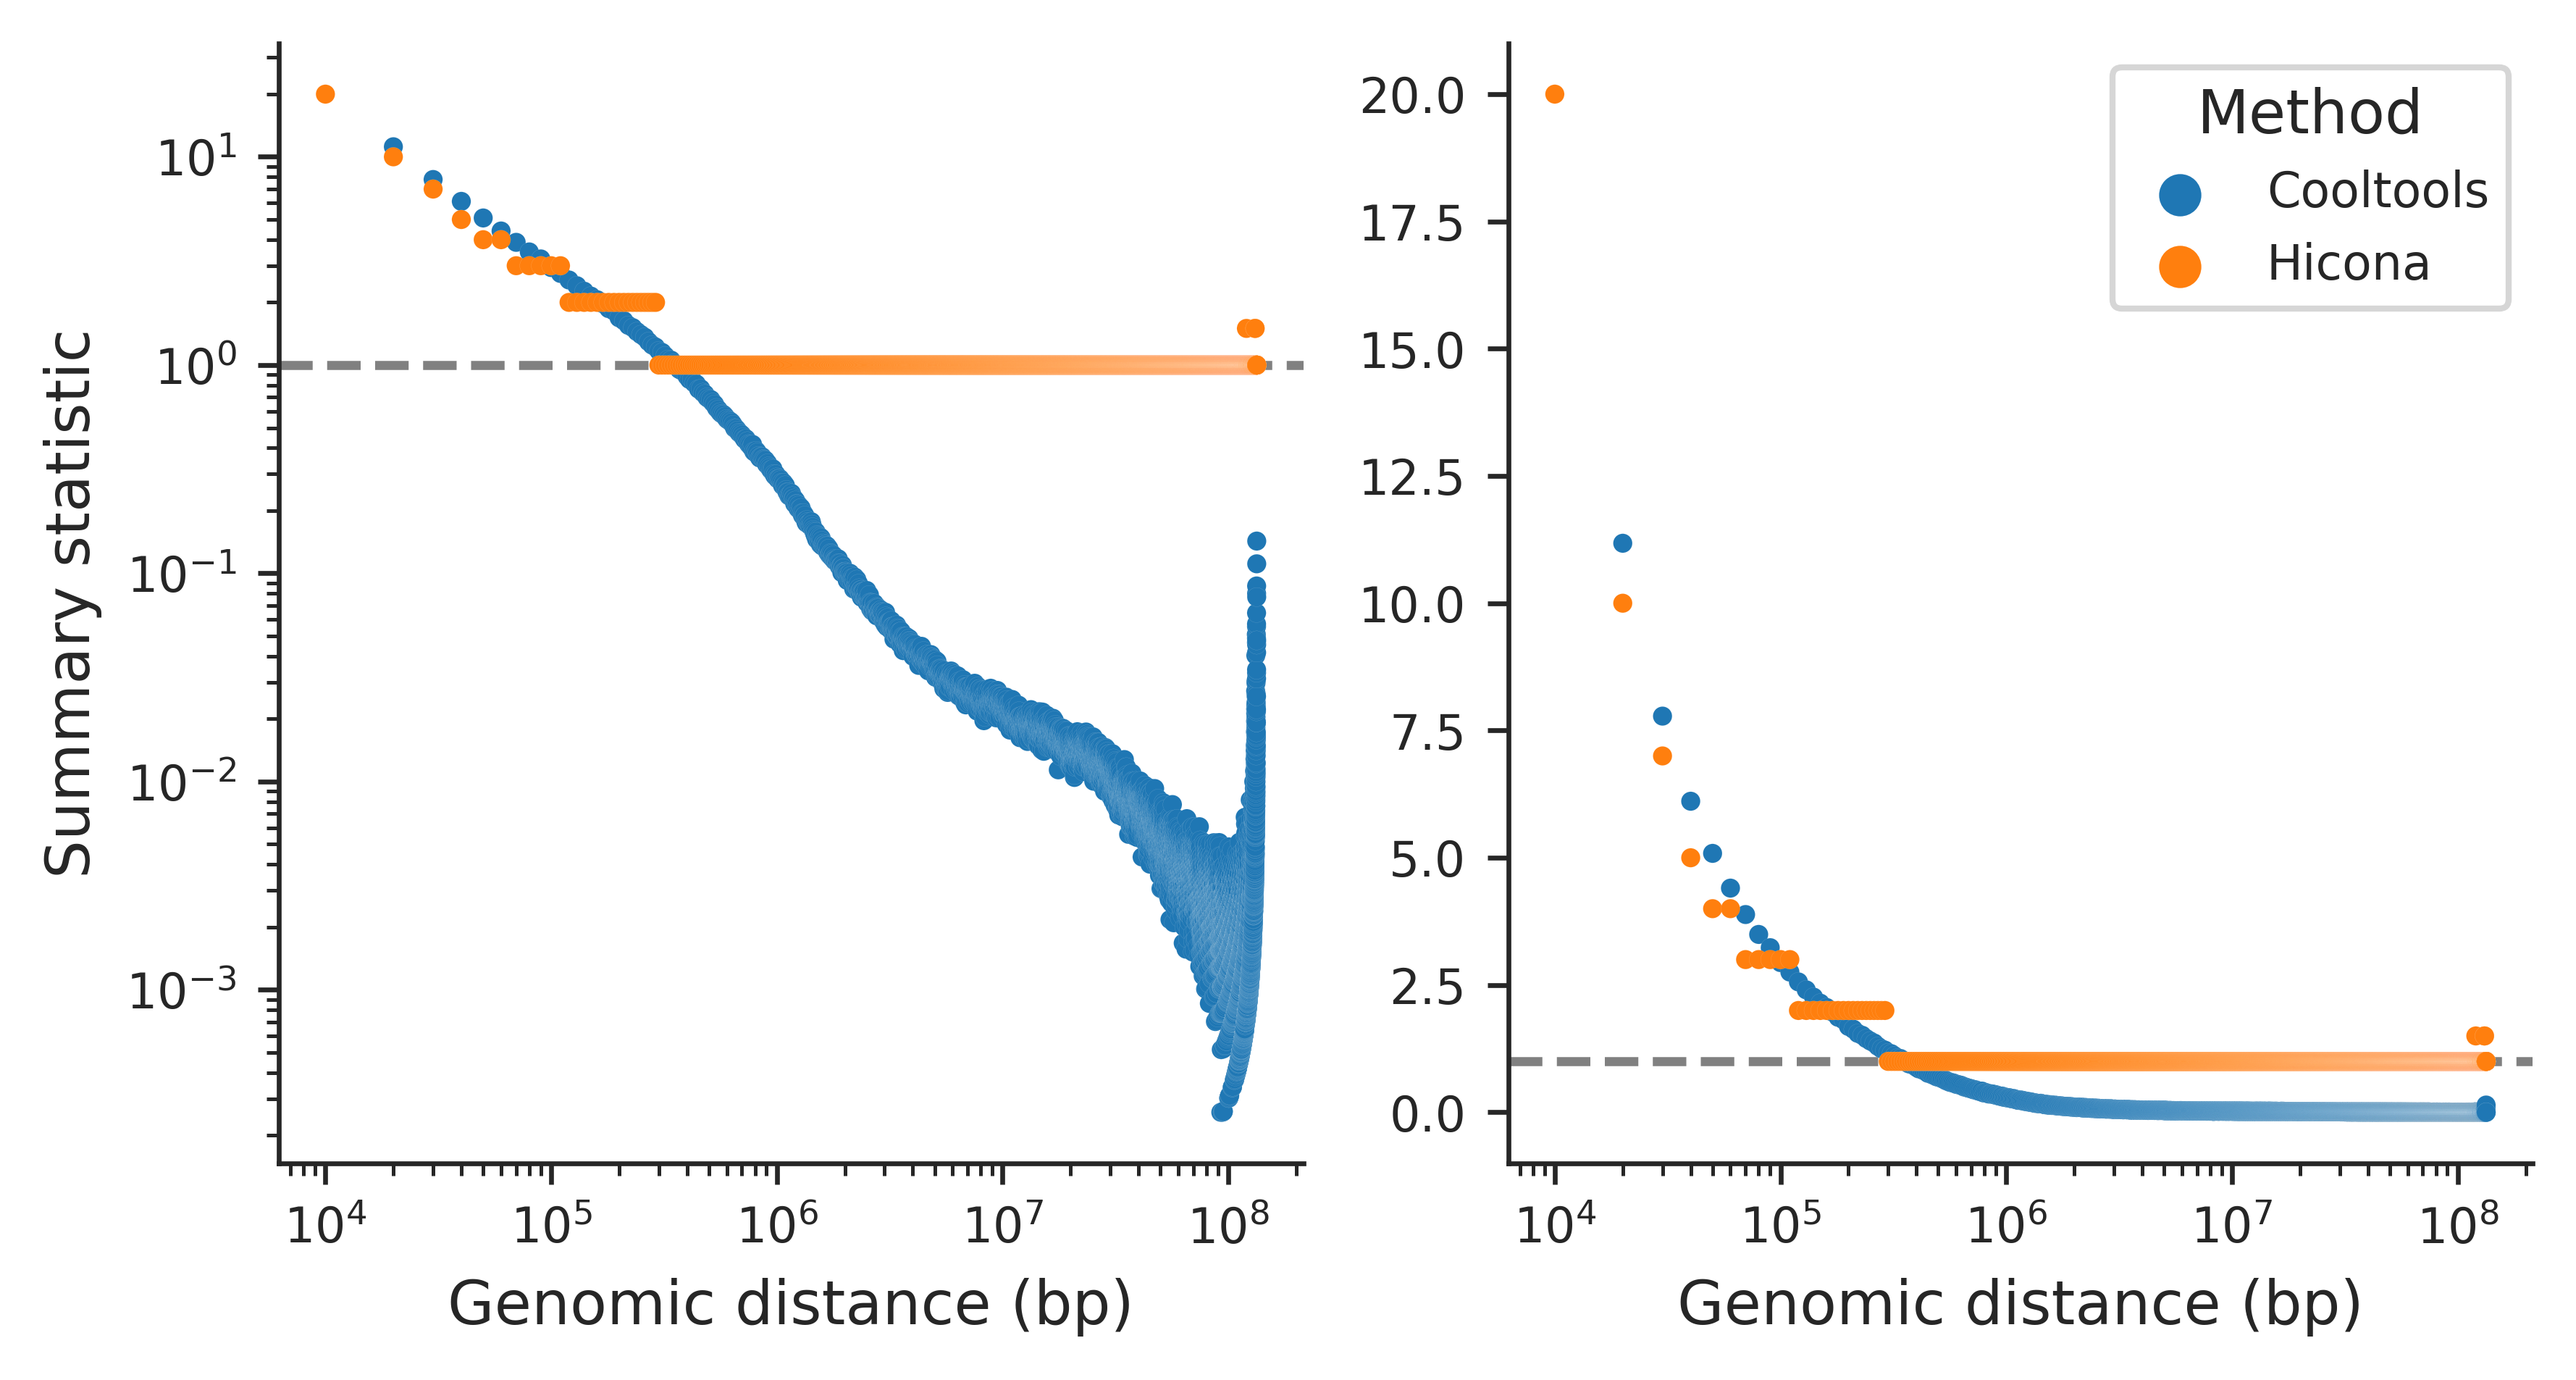
\includegraphics[width=1\textwidth]{hicona_vs_cooltools.png}
  \caption{\textbf{Comparison of summary statistics from HiCONA and cooltools}. Comparison of the genomic distance normalization factors for chromosome 1 of IMR90 cells, filtered using 200 Mb as genomic distance threshold, obtained using HiCONA and cooltools. On the left, normalization factor with respect to distance in log-log scale, on the right same plot but without log-transform of the y-axis. Replicates with different files and chromosomes are in appendix [ADD REF]}
  \label{fig:cooltools}
\end{figure}

As previously mentioned, the probability of two genomic regions interacting by chance decays exponentially with their distance from each other; for this reason, we also expect the function describing probability of contact given distance to be linear in a log-log plot. As shown in the left panel of figure \ref{fig:cooltools}, the summary statistic provided by cooltools can indeed be considered linear for a big range of genomic distances (up to $10^7$ bp); for very high distances though, we start observing some fanning which represents instability due to the low number of pixels averaged. This happens not only because the number of interactions decays with distance, but also because the number of theoretically possible pixels decreases. Visually, increasing distance means moving from the main diagonal of the contact matrix to diagonals closer to the upper right corner, which become shorter and shorter. Cooltools allows to address this instability with a smoothing procedure, though it currently requires matrix balancing, which introduces the assumption that all genomic loci form the same number of contacts. In synthesis, the procedure adopted by cooltools is biologically sensible, though it has some drawbacks such as very low counts and instability at very high distances.


The summary statistic proposed by HiCONA, instead, is not linear in the log-log plot. At low distances it behaves similarly to cooltools, but then it plateaus at 1 (or if a minimum count threshold is imposed, the cutoff itself becomes the plateau value). Though at first glance the two methods seem rather different, this is mostly due to the logarithmic scale of the y-axis. The right panel of figure \ref{fig:cooltools} represents the same plot but with the y-axis in linear scale; from this we notice that the values provided by the two methods are actually quite close, since cooltools tends asymptotically to 0, while HiCONA is stable at 1 (with some rare exceptions at extremely high distances). Moreover, it must be considered that non-normalized pixel counts are integers strictly greater than zero, therefore the minimum value which they can take is 1; by using a number close to zero as summary statistic, and thus to compute a fold change, a pixel with count 1 at high distance will seem extremely significant, though it might be due to a single random ligation event. The statistic provided by HiCONA is therefore similar to the biologically motivated one provided by cooltools, though with the advantage of being more stable and yielding integer values.


When processing a file with a specific set of filtering parameters, regardless of the usage of cooltools or HiCONA, one summary statistic function is computed for each individual chromosome. This is done to avoid relying on the assumption that random contact probability decays at the same rate in all chromosomes. One might argue that considering all pixels jointly would yield a more robust and less noisy function; while that would indeed be the case, each chromosome has enough pixels to obtain a robust result on its own (aside from chromsome Y due to its significantly smaller size and probably other biological motivations).


\subsection{Genomic distance normalization}

After computing the normalization factors, the pixels are normalized by taking the $\log_2$ of 1 plus the ratio between raw count value and normalization factor. This means that pixels whose count is equal to the expected one will have normalized value equal to 1; moreover, any value above 1 represents a pixel with higher count than the expected, any value below 1 represents a pixel with lower count than expected. 

% Plot from first lab meeting with distribution prior and after normalization
\begin{figure}[ht]
  \centering
  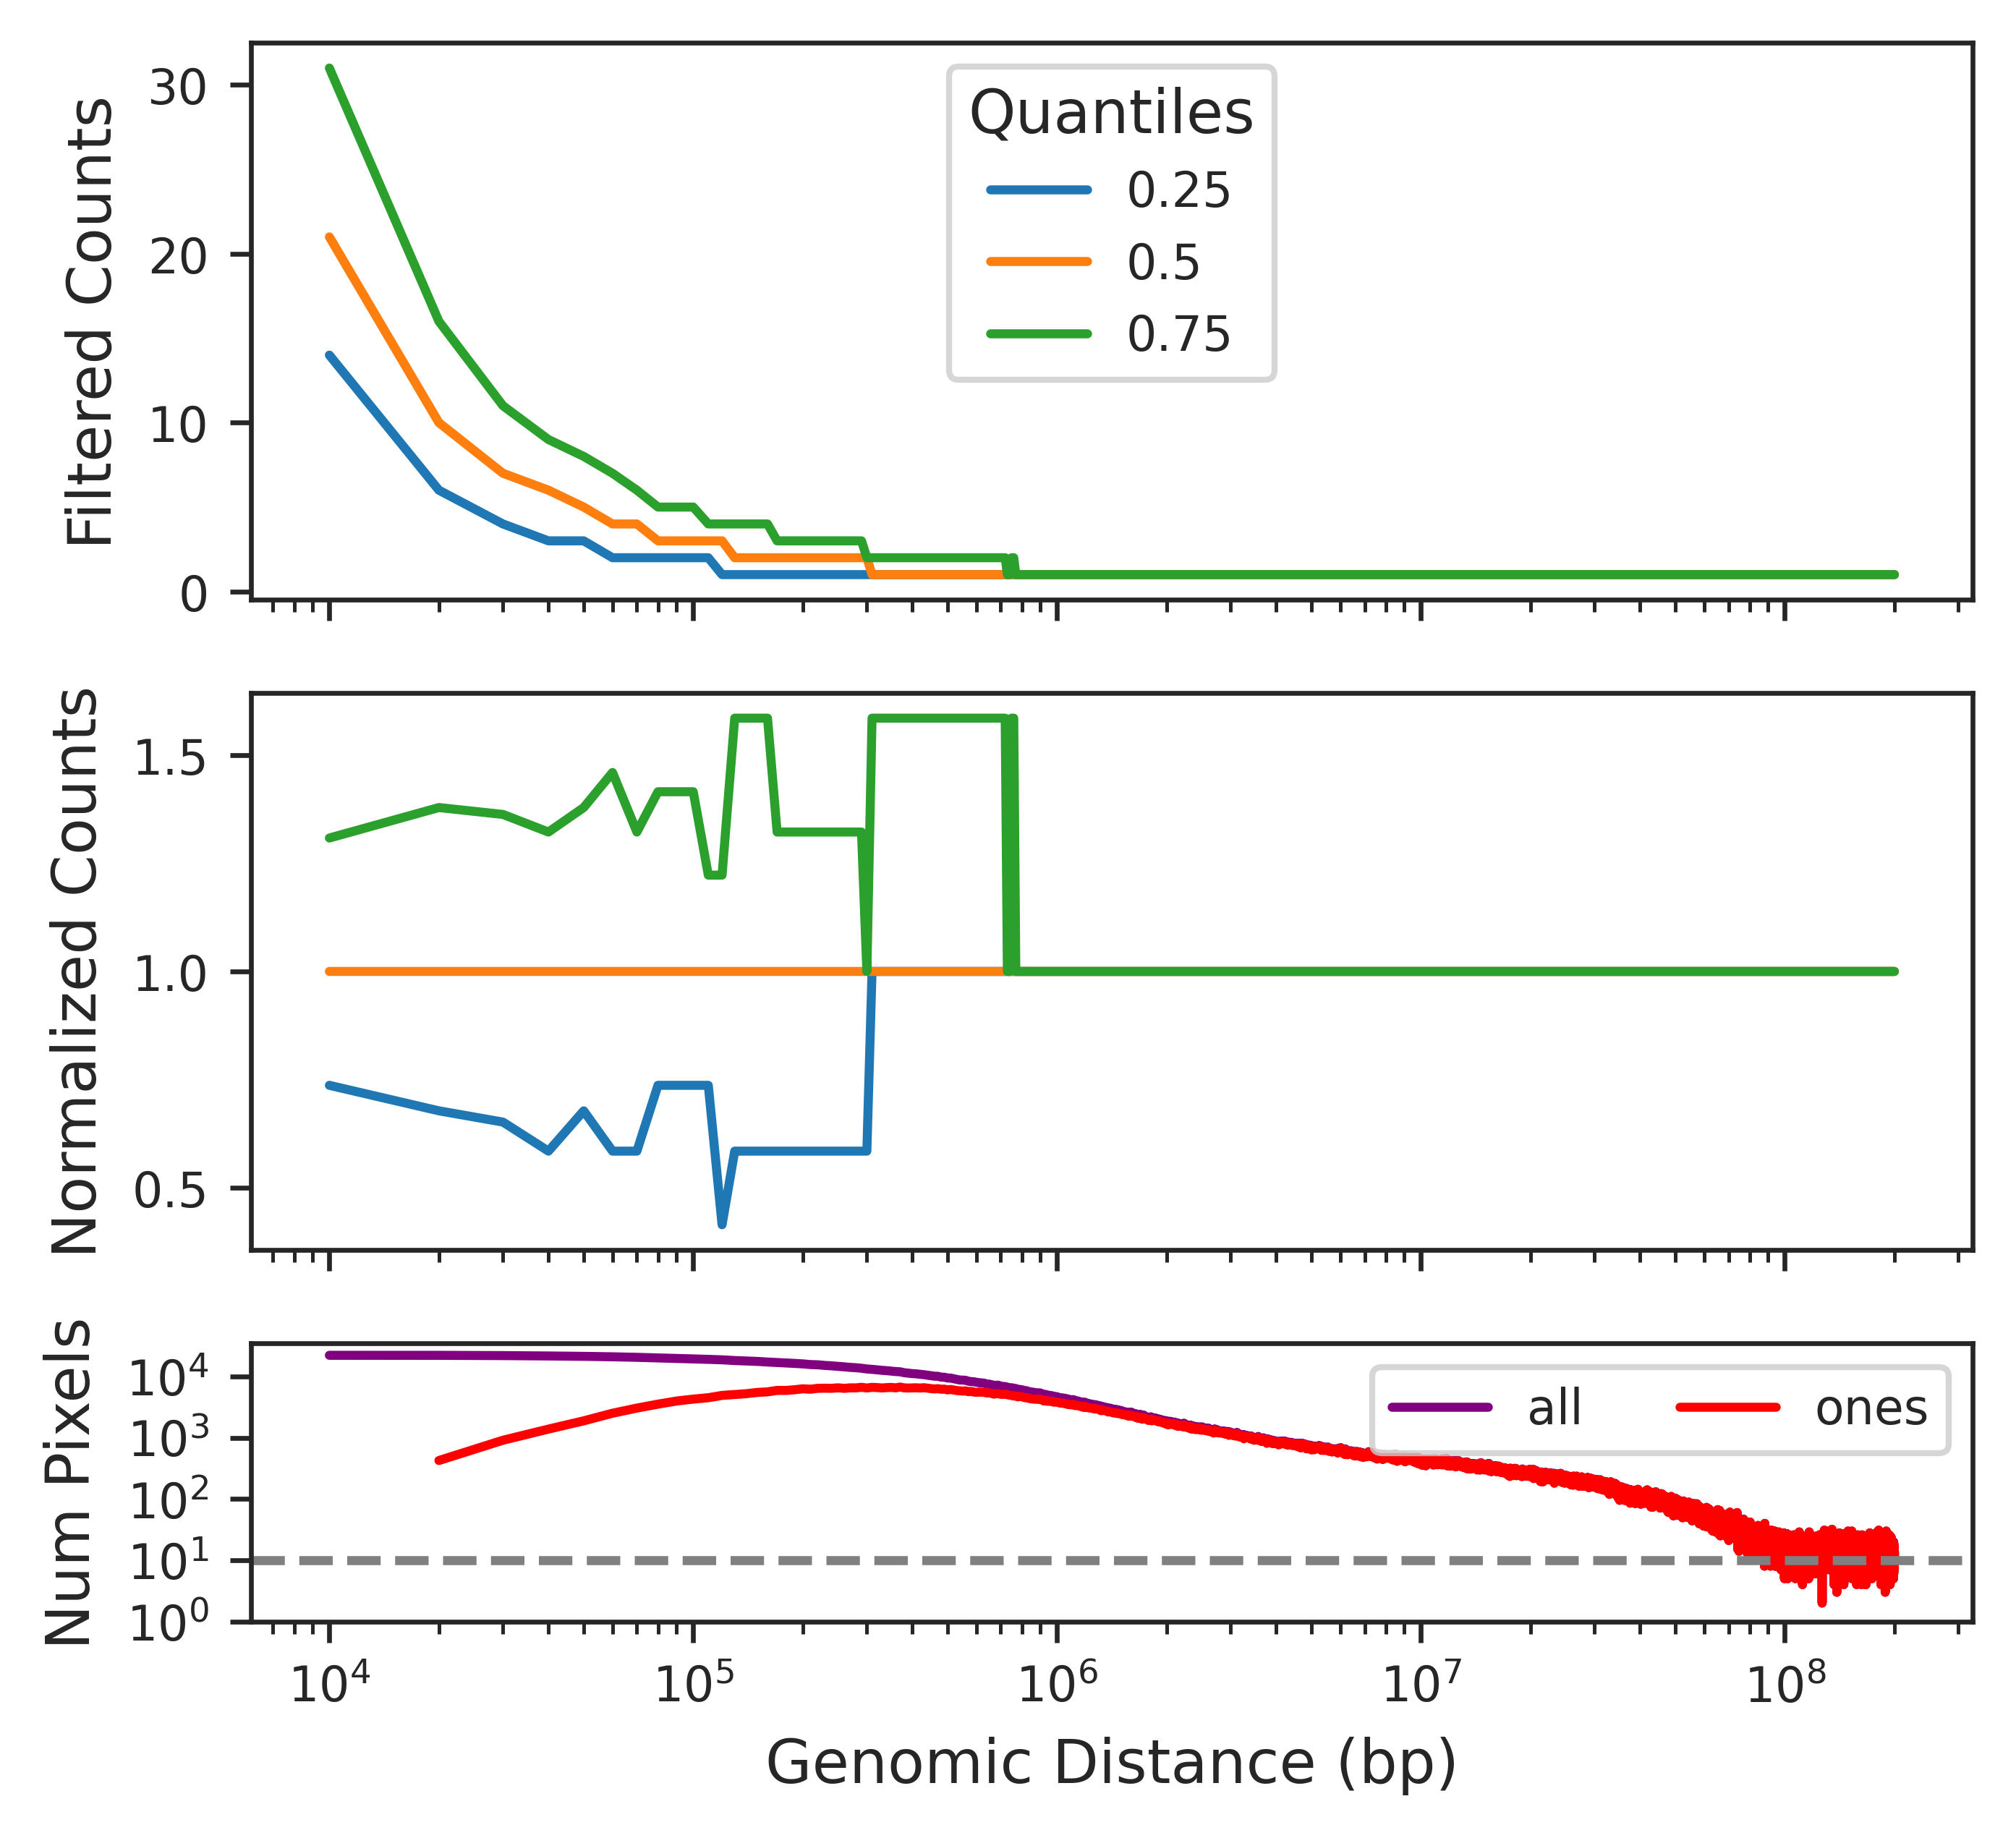
\includegraphics[width=0.8\textwidth]{normalization_stats.png}
  \caption{\textbf{Comparison of pixels counts distribution prior and post genomic distance normalization}. Comparison of the distribution of raw and normalized counts at each genomic distance for chromosome 1 of IMR90 cells, filtered using 200 Mb as genomic distance threshold. At the top, quantiles of the raw counts distribution for each genomic distance. In the middle, quantiles of the normalized counts distribution for each genomic distance. At the bottom, total number of pixels, and number of pixels with raw count equal to 1, for each genomic distance.}
  \label{fig:normstats}
\end{figure}

In figure \ref{fig:normstats} we can observe how the counts distribution changes with normalization. In the top panel, the quantiles of the raw counts distribution for each genomic distance are shown. Though the median of the raw counts distribution can start at different values, in this case 22, it always quickly converges to 1. This behviour can also be justified by looking at the bottom panel, which shows the total number of pixels, and the number of pixels with raw count equal to 1, in function of genomic distance. While the number of pixels quickly decreases with distance, to the point where there are less then 100 at $10^8$ bp, the fraction of them with raw count equal to 1 rapidly increases; at $10^6$ bp, basically all pixels have raw count equal to 1, thus motivating the median being equal to 1. In the middle panel, the quantiles of the normalized counts distribution for each genomic distance are shown. As one might expect from a normalization process, the value of the median is always 1. Even though the high fraction of raw counts equal to 1 makes it less obvious, on closer inspection it can be seen that the regularitazion of the spread actually works quite well. Up to $2 \cdot 10^5$ bp, there is a spread in the normalized counts distributions of up to $0.6$ units in either direction of the median. Then, from $2 \cdot 10^5$ to $8 \cdot 10^5$ bp, the same spread of $0.6$ points is present, though only in the positive direction. This it is due to the fact that, at these distances, more than half of the raw counts are equal to 1, as highlighted by the bottom panel and the median in the top one being 1; since 1 is the minimal value that raw counts can take, it means there there are no pixels who can have a raw count below the expected one, and thus a normalized value lower than 1. After $8 \cdot 10^5$ bp, almost all the pixels have raw count equal to 1, thus all quantiles are equal to 1; for this reason it is still impossible to have values lower than 1, and while normalized values above 1 are possible, they are so rare that they do not alter the position of the quantiles. All of this to say that, when there is a sufficient amount on pixels with raw count different from 1 to allow for non overlapping quantiles, the amplitude of the spread falls within a very consistent range of one point in either direction, with few distances exceeding this range (regardless of chromosome, cell type, filtering parameters or file size). 


A relevant fact to consider regarding the normalized values is that, though normalized counts are floating point numbers, they are obtained by taking the $\log_2$ of a fraction whose terms are integers; not only that, the values which the denominator can take are rather limited, very rarely exceeding 100. For this reason, in actualty, the pool of normalized values is smaller than it might seem and this becomes relevant during sparsification since repeated values allow for the use of memoization in order to speed up computations.

\subsection{Pixel filtering}

The preliminary step of pixel filtering is to remove inter-chromosomal pixels. As explained in subsection \ref{par:pixfiltering}, this is because it is not possible to define genomic distance across chromosomes, and therefore these pixels cannot be processed in a comparable way with respect to the intra-chromosomal ones. This step removed, on average, 53.27\% of pixels from the files at 10 kb resolution, 45.62\% of pixels from those at 5 kb resolution.

All the intra-chromosomal pixels for a single chromosome can then be filtered. Firstly, self-looping pixels are removed. Then, pixels with genomic distance above a specified threshold are removed. Ideally one would set a threshold which corresponds to the maximal distance for a biologically relevant interaction; this value has not yet been defined, hence educated guesses and trial and error are the only real choices for now. Filtering using a count threshold was not performed since it was not required. After these steps, the partially filtered chromosome-level table can be normalized as discussed in the previous subsection. The normalized table can be then optionally filterd using a quantile threshold: the value corresponding to a specified quantile of the normalized counts is computed, then all pixels whose normalized counts value is equal to or below it are removed. Once again, this threshold still has to be defined empirically. 

In figure \ref{fig:filtering}, some chromosome filtering statistic, aggregated by file, are shown. In each of the panels, the boxes are divided in groups, each one corresponding to a genomic distance threshold, which were sorted from left to right by increasing strictness. Within each group of boxes, each box corresponds to a quantile threshold, once again sorted from left to right in each group by increasing strictness.

In the top panel, the fraction of retained intra-chromosomal pixels after filtering is reported. As expected, both decreasing the distance threshold and increasing the quantile threshold, therefore making the filtering conditions more strict, lead to a decrease in the fraction of retained pixels. While changing distance threshold yields gradual changes in the fraction of retained pixels, changing quantile threshold can cause a quite abrupt drop. This is due to the fact that many pixels, if not most of them, have normalized counts equal to 1. To exemplify this, consider the hypothetical case in which two very distant quantiles, say 0.25 and 0.75, both correspond to a normalized value of 1 due to the sheer number of pixels with that nomarlized counts value; trying to filter using quantile threshold 0.25 would mean removing all pixels with normalized counts equal to 1, which in turn results in removing all pixels up to the quantile threshold 0.75 since those have normalized counts equal to 1 too, thus causing a drop similar to the one observed in the plot.

In the middle panel, the fold change between the mean genomic distance of the filtered pixels and the mean genomic distance of the non filtered ones is shown. In the bottom panel, the same fold change is represented but using the median instead of the mean. As one might expect, a reduction in both mean and median is observed, which gets progressively bigger as the distance threshold gets smaller. Quantile threshold does not seem to have a big impact on mean and median distance reduction, aside from the drop between 0.05 and 0.1 which is due to the previously mention drastic reduction in pixel number. The spread of the mean fold change for a single combination of parameter is quite small, while the spread of the median fold change is quite big; altough the spread in median fold change might be due to actual differences in the distribution of genomic distances in the different samples, it is more likely that it is simply due to the way the measure is computed, since it is the ratio among two individual data points (while in the case of the mean, both numerator and denominator are the average of millions of data points).

\begin{figure}[ht]
  \centering
  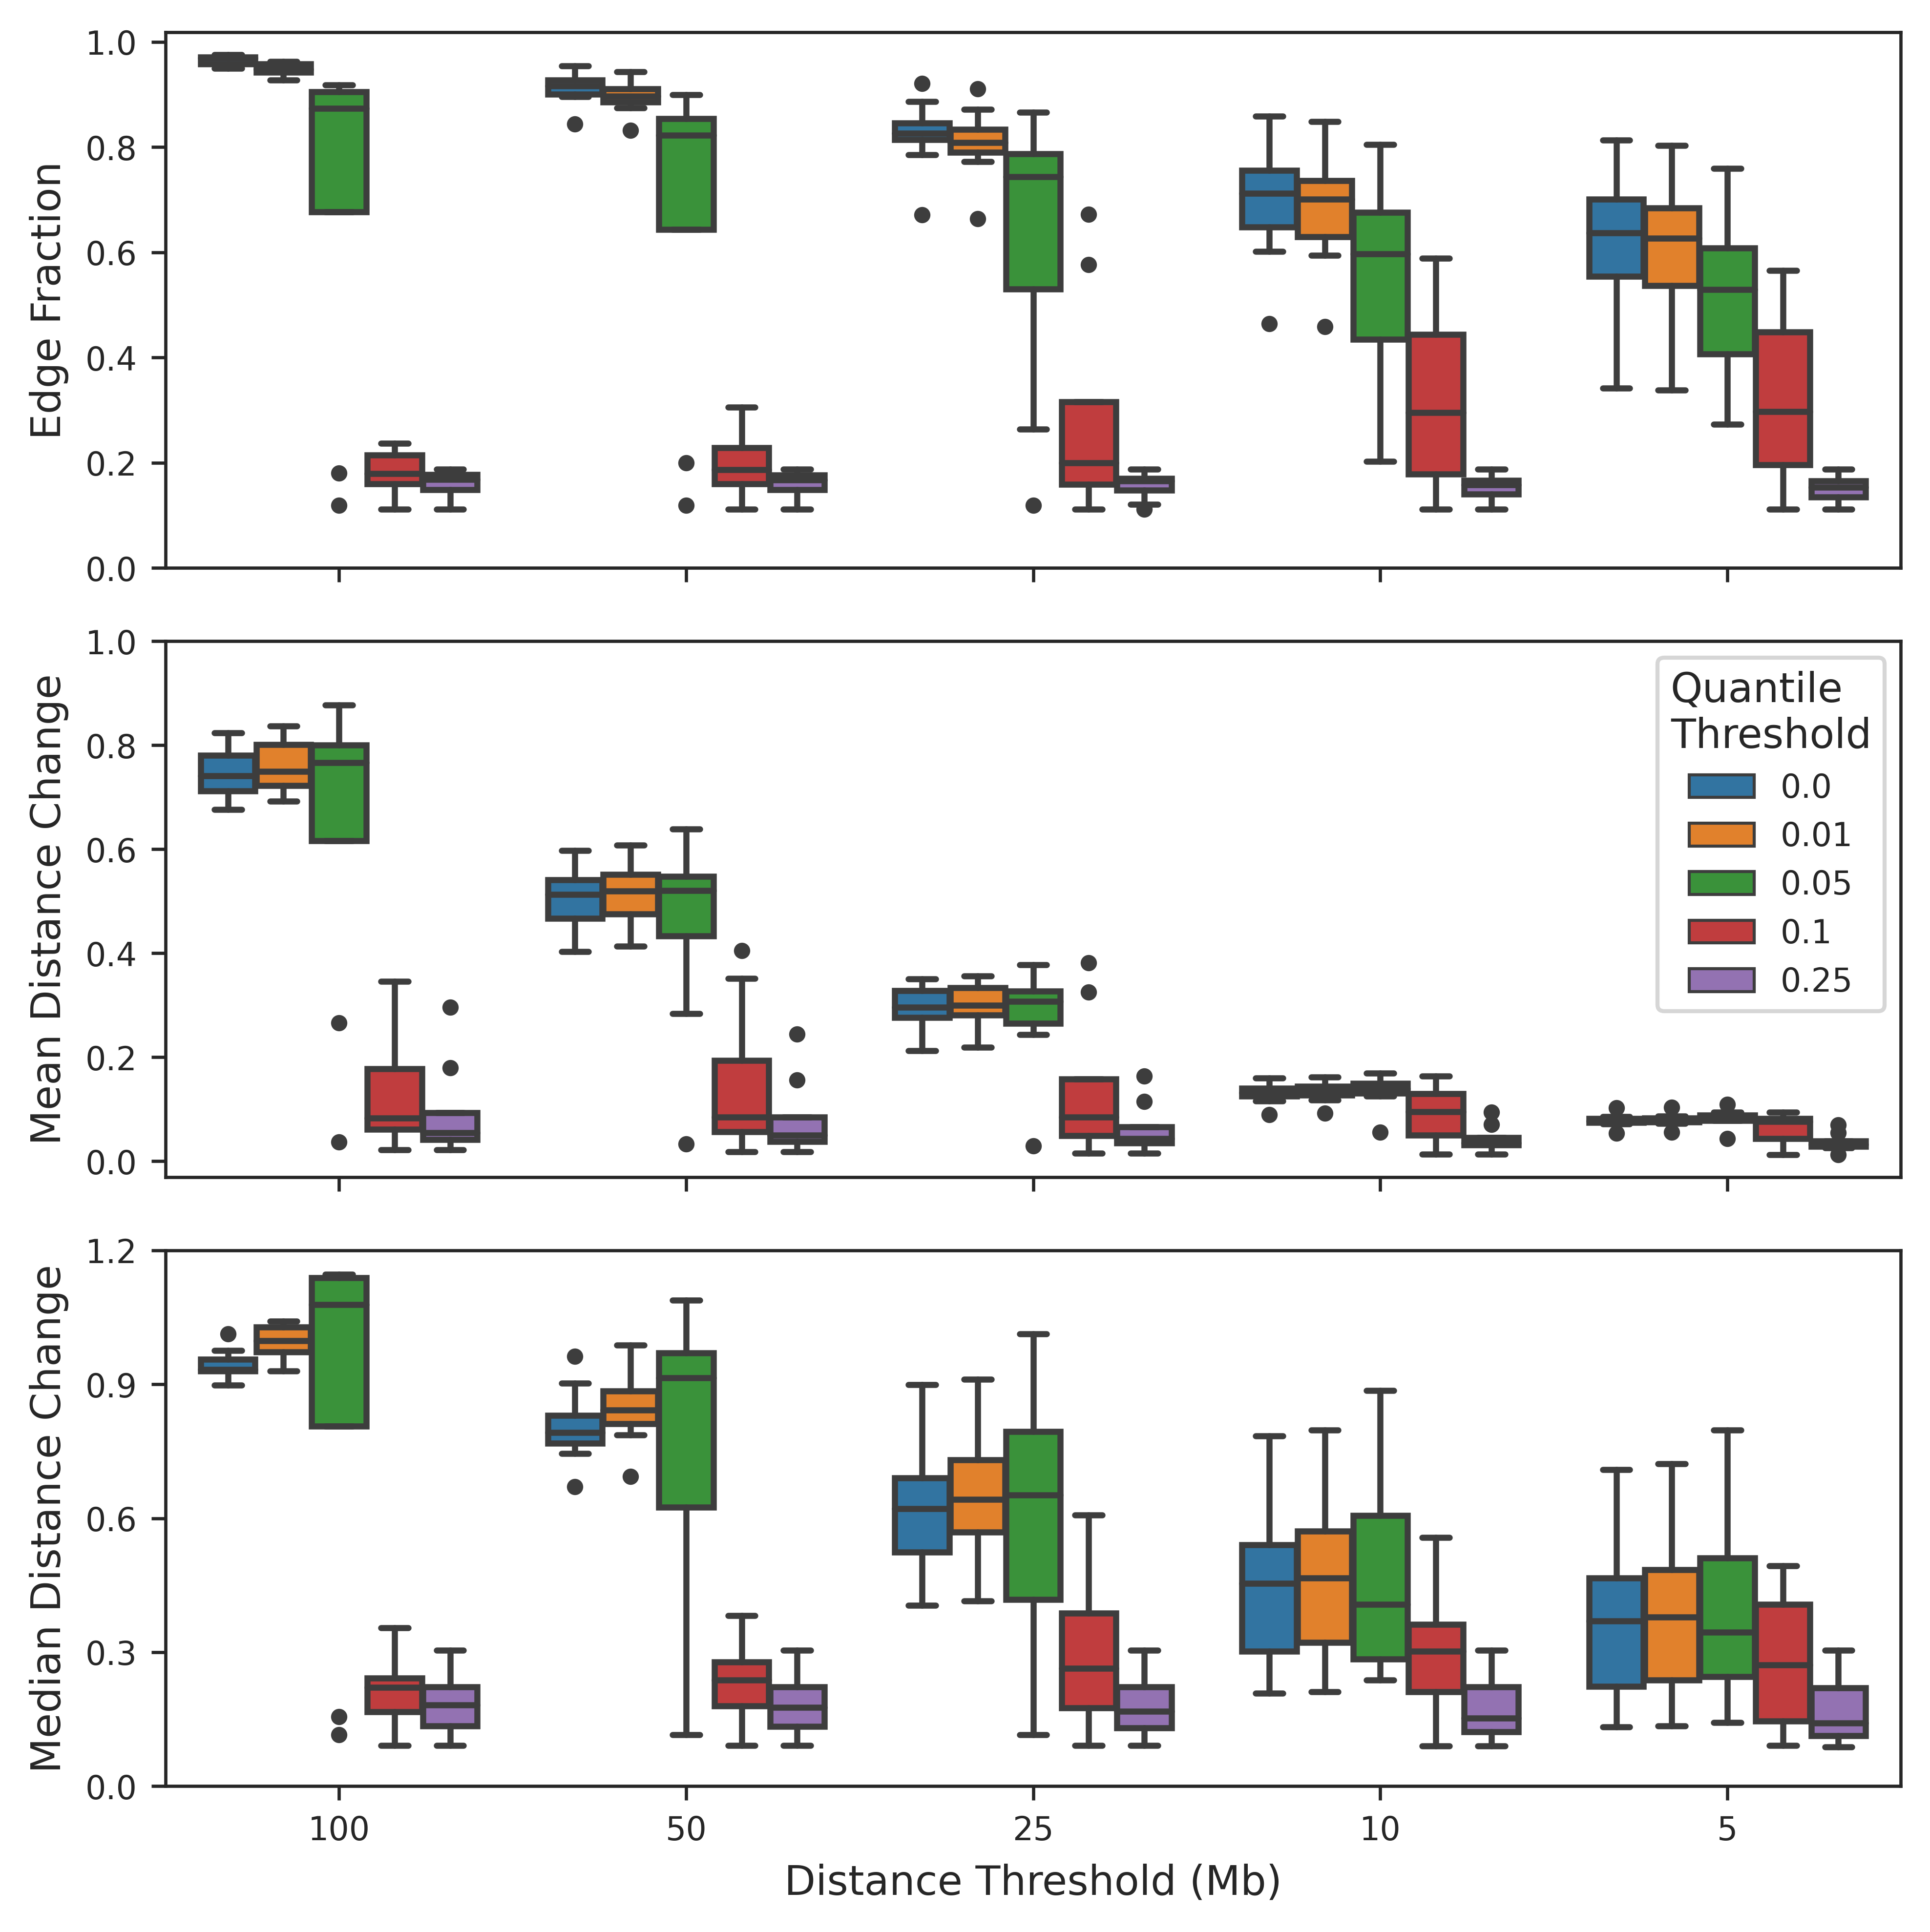
\includegraphics[width=0.8\textwidth]{filtering_stats.png}
  \caption{\textbf{Changes in pixel number and distance statistics after filtering}. Comparison of the changes in edge number and distance statistics using different filtering parameters on all eight main cool files. Each group of boxes corresponds to one distance threshold, which are sorted from left to right, from least stringent to most stringent. Each box in a group corresponds to one quantile threshold, and within a group, boxes are sorted from left to right, from least stringent to most stringent. At the top, fraction of intra-chromosomal pixels remaining after filtering. In the middle, fold change between filtered pixels mean genomic distance and intra-chromosomal pixels mean genomic distance. At the bottom, fold change between filtered pixels median genomic distance and intra-chromosomal pixels median genomic distance}
  \label{fig:filtering}
\end{figure}

The ideal combination of parameters to use for filtering is one that allows to reduce the number of pixels while impacting minimally mean and, especially, median distance fold changes, or at least affecting them in a consistent way (that is, lower spread in the filtering statistics). Given these premises, the only parameter values which seem appropriate are 0.0 and 0.01 for quantile threshold and 100 Mb and 50 Mb for the distance threshold. It is though worth noting that 0.0 and 0.01 quantile threshold belong almost identically and that 0.0 correspond to non applying the filter at all; moreover both 100 Mb and 50 Mb are still very permissive thresholds in terms of genomic distance. This indicates that this filtering step is not doing much, and it could probably be removed altogether (aside from the removal of self looping pixels and inter-chromsomal ones). From here on, the files are always assumed to have been filtered using a combination of the parameters deemed viable.


\subsection{Optimal alpha computation}

After pixel filtering, the sparsification scores (alpha values) are computed for each pixel as discussed in subsection \ref{par:sparscore}. HiCONA computes and stores both alpha values for each edge, in order to be able to used either the minimum or the maximum of the two. To perform the actual sparsification, an alpha cutoff must be defined, either an arbitrary one or the one defined by HiCONA as optimal, that is the chromosome-level threshold which minimizes the number of edges while maximising the number of nodes. This value is computed using a local search algorithm; one example of the grid of values tested by a run of the local search in shown in figure \ref{fig:alphas}.

For each chromosome the local search is actually run twice, one using the minimal alphas, one using the maximal ones
Typically, the minimum and the maximum alpha thresholds for the same chromosome are almost always different, though they still tend to be very close to each other. The typical range for the optimal alpha values is between 0.15 and 0.30. Chromosome Y is an exception. 

% Plot alpha computation grid for some file (maybe multiple sets of params)
\begin{figure}[h]
  \centering 
  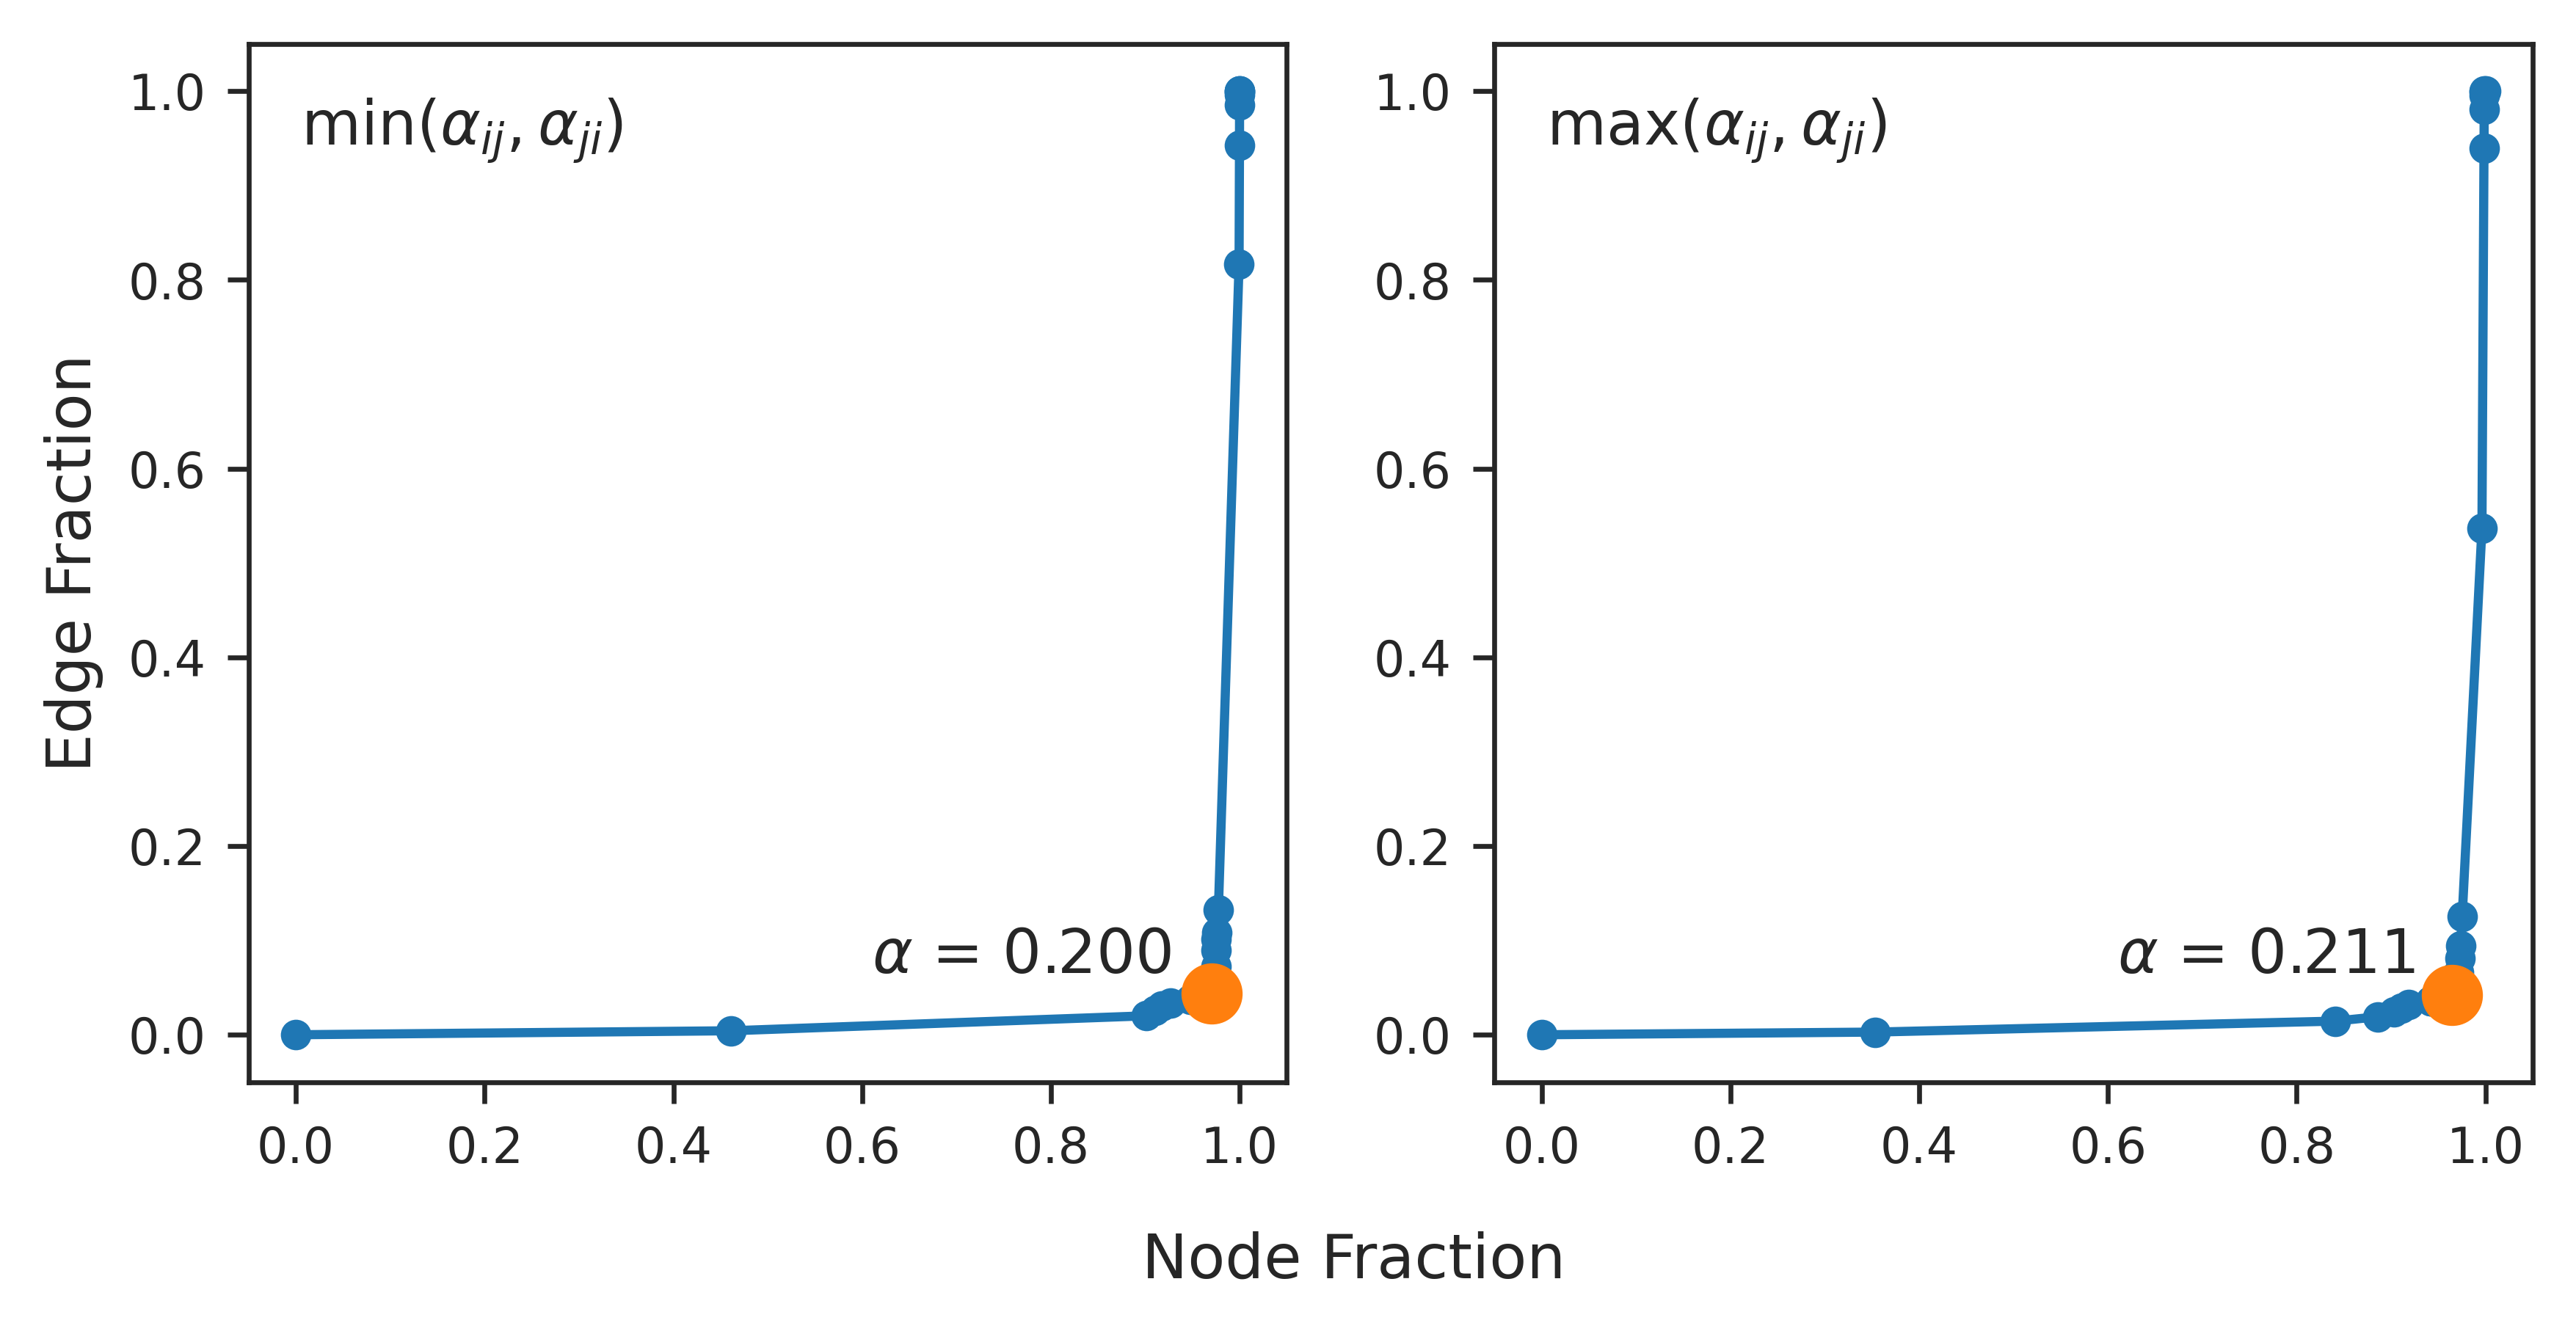
\includegraphics[width=1\textwidth]{alpha_tables.png}
  \caption{\textbf{Optimal alpha selection process}. To define the optimal alpha value to sparsify the chromosome-level network, local search is performed. On the left, set of points tested while trying to find the optimal alpha value for chromosome 1 of IMR90 cells, sparsified using... }
  \label{fig:alphas}
\end{figure}

\subsection{Pixel sparsification}
% Plot number of pixels as function of parameters
% Plot variation coefficient with other tools too
% Plot distance of pixels as function of parameters
% Plot expected interaction distance with respect to other tools


\section{Pixel preprocessing performance}

\subsection{Time benchmark}
% Plot number of filtered pixels vs time (linear)
\subsection{Memory benchmark}
% Plot of the run of a single file using memprof

\section{Pixel preprocessing biological validation}

\subsection{Consistency on replicates}
% Plot Jaccard index on replicates 
% Plot Jaccard index vs file size pre and after processing
% Plot Jaccard index with respect to other tools

\subsection{Functional annotations enrichment}
% Plot edge annotation fraction
% Plot edge annotation enrichment



% \section{Network analysis}
% \subsection{Node-label permutations}
% Plot node-label permutation for 1 file, chromosome-wise (maybe new ann)

% ? Plot Hi-C maps at different steps
% TODO: Maybe use in memory benchmarking
% It follows that the reported file size is then 20 bytes times the number of rows of the pixel table. Since two columns of the pixel table ("bin1\_id" and "bin2\_id") are vectors of 64-bit signed integers, while the remaining one ("count") is a vector of 32-bit signed integers, each row of the pixel table requires 20 bytes of memory.